% One policy question answered with RAG (phase 2, POST /api/ask).
% Build: tectonic --outdir . fig-rag-flow-v1.tex
\documentclass[border=16pt]{standalone}
\usepackage[T1]{fontenc}
\usepackage[utf8]{inputenc}
\usepackage{helvet}
\renewcommand{\familydefault}{\sfdefault}
\usepackage[none]{hyphenat}
\usepackage{tikz}
\usetikzlibrary{arrows.meta,calc,shapes.geometric}

\definecolor{ink}{HTML}{0F2A33}
\definecolor{muted}{HTML}{5E7078}
\definecolor{line}{HTML}{C3CED2}
\definecolor{blue}{HTML}{1F5FA8}
\definecolor{orange}{HTML}{E2551F}
\definecolor{hubfill}{HTML}{EDF2F4}

\newcommand{\lbl}[2]{\textbf{#1}\\[2pt]{\footnotesize\color{muted}#2}}

\begin{document}
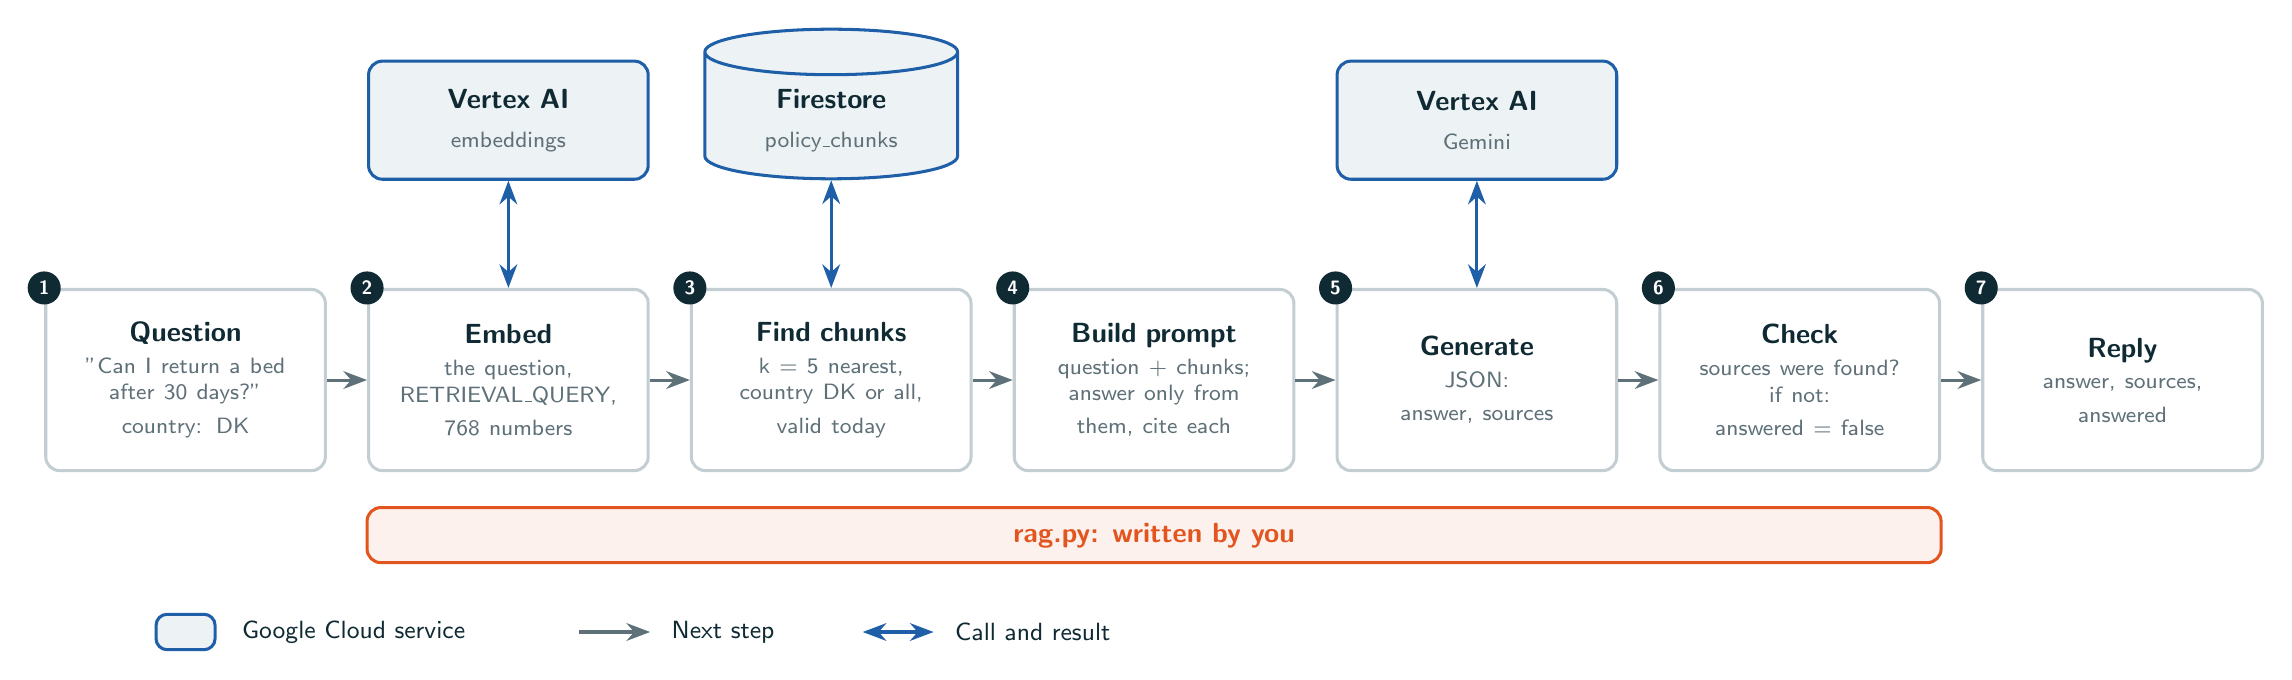
\begin{tikzpicture}[
  font=\sffamily,
  box/.style={rounded corners=5pt, draw=line, line width=1.1pt, fill=white,
    text=ink, align=center, text width=3.2cm, minimum height=2.3cm,
    inner sep=5pt},
  gcp/.style={box, draw=blue, fill=hubfill, minimum height=1.5cm},
  store/.style={cylinder, shape border rotate=90, aspect=0.18,
    draw=blue, fill=hubfill, line width=1.1pt, text=ink, align=center,
    text width=3.0cm, minimum height=1.9cm, inner sep=3pt},
  one/.style={line width=1.1pt, draw=muted, -{Stealth[length=3mm]}},
  two/.style={line width=1.1pt, draw=blue,
    {Stealth[length=3mm]}-{Stealth[length=3mm]}},
  num/.style={circle, fill=ink, text=white, font=\scriptsize\bfseries,
    inner sep=1.2pt, minimum size=0.42cm},
]

\def\dx{4.1}

% ---- The row of steps ----
\node[box] (q) at (0,0)
  {\lbl{Question}{"Can I return a bed\\after 30 days?"\\country: DK}};
\node[box] (emb) at (\dx,0)
  {\lbl{Embed}{the question,\\RETRIEVAL\_QUERY,\\768 numbers}};
\node[box] (ret) at (2*\dx,0)
  {\lbl{Find chunks}{k = 5 nearest,\\country DK or all,\\valid today}};
\node[box] (pr) at (3*\dx,0)
  {\lbl{Build prompt}{question + chunks;\\answer only from\\them, cite each}};
\node[box] (gen) at (4*\dx,0)
  {\lbl{Generate}{JSON:\\answer, sources}};
\node[box] (chk) at (5*\dx,0)
  {\lbl{Check}{sources were found?\\if not:\\answered = false}};
\node[box] (ans) at (6*\dx,0)
  {\lbl{Reply}{answer, sources,\\answered}};

\foreach \a/\b in {q/emb, emb/ret, ret/pr, pr/gen, gen/chk, chk/ans}
  \draw[one] (\a.east) -- (\b.west);

\foreach \n/\k in {q/1, emb/2, ret/3, pr/4, gen/5, chk/6, ans/7}
  \node[num] at (\n.north west) {\k};

% ---- Services above the row ----
\node[gcp] (vx) at (\dx,3.3)
  {\lbl{Vertex AI}{embeddings}};
\node[store] (fs) at (2*\dx,3.3)
  {\lbl{Firestore}{policy\_chunks}};
\node[gcp] (gm) at (4*\dx,3.3)
  {\lbl{Vertex AI}{Gemini}};
\draw[two] (emb.north) -- (vx.south);
\draw[two] (ret.north) -- (fs.south);
\draw[two] (gen.north) -- (gm.south);

% ---- Band: the part you write ----
\draw[orange, line width=1.1pt, rounded corners=5pt, fill=orange!8]
  ($(emb.south west)+(0,-0.45)$) rectangle ($(chk.south east)+(0,-1.15)$);
\node[text=orange, font=\bfseries] at
  ($($(emb.south west)+(0,-0.8)$)!0.5!($(chk.south east)+(0,-0.8)$)$)
  {rag.py: written by you};

% ---- Legend ----
\node[rounded corners=4pt, draw=blue, line width=1.1pt, fill=hubfill,
      minimum width=0.75cm, minimum height=0.45cm] (k1) at (0,-3.2) {};
\node[anchor=west, text=ink, font=\small] at ([xshift=0.2cm]k1.east)
  {Google Cloud service};
\draw[one] (5.0,-3.2) -- (5.9,-3.2);
\node[anchor=west, text=ink, font=\small] at (6.05,-3.2) {Next step};
\draw[two] (8.6,-3.2) -- (9.5,-3.2);
\node[anchor=west, text=ink, font=\small] at (9.65,-3.2) {Call and result};

\end{tikzpicture}
\end{document}
